\documentclass[main.tex]{subfiles}
\begin{document}
\section{Architectural Strategy}
The architectural strategy presents two quality attributes of YANF that are described with the use of Quality Attribute Scenarios (QAS) and how they are realized with the use of tactics. Each subsection argues for the exact choice of a given tactic.

%The terms used in the scenarios are described in \autoref{lst:privacyScenarioTerms}.

%\begin{figure}[H]
%    \centering
%    \begin{itemize}
%        \item \textbf{Mobile phone app} - any application on the phone that communicates over the network with HTTP
%        \item \textbf{Local VPN service} - VPN server and client running on the mobile phone in the background
%        \item \textbf{Destination} - receiver of a HTTP-request (a server)
%    \end{itemize}
%    \caption{Privacy scenario terms}
%    \label{lst:privacyScenarioTerms}
%\end{figure}

\subsubsection{Privacy QAS \& Tactic}
\label{subsec:PrivacyTacticandScenario}
User story (US1, \autoref{tab:user_stories}) describes a functionality where cookies should be removed from HTTP requests to avoid tracking from 3\textsuperscript{rd} parties. The tactic \textit{Protection against Tracking} from \hyperlink{PrivacyPatterns.org}{PrivacyPatterns.org}\cite{UCBerkeley-SchoolofInformationProtectionPatterns} describes this issue in more detail. In this case the user story and the tactic are very alike but the difference is that the tactic should describe when cookies should be removed from the HTTP requests. For this application the cookies should be removed on a blacklist basis where untrusted parties are not allowed to retrieve cookies from the user. \Autoref{tab:PrivSce} lists the QAS for handling cookies sent by the mobile phone. \textit{Normal mode} simply means that the application is blocking cookies in real-time depending on a list of blacklisted domains i.e. the disconnect.me-list.

\begin{table}[H]
    \centering
    \begin{tabular}{|p{5cm}|p{8cm}|} \hline
        \textbf{Portion of Scenario}& \textbf{Values}   \\ \hline
        Source                      & Mobile phone app  \\ \hline
        Stimuli                     & HTTP-request containing a cookie in the header    \\ \hline
        Artefact                    & Local VPN Service, Destination server  \\ \hline
        Environment                 & Normal mode       \\ \hline
        Response                    & Cookie is excluded from HTTP request  \\ \hline
        Response Measure            & HTTP-request header contains no cookie\\ \hline
    \end{tabular}
    \caption{QAS Privacy}
    \label{tab:PrivSce}
\end{table}


\subsubsection{Energy Efficiency QAS \& Tactic}
\label{subsec:EnergyEfficiencyTacticandScenario}
User story (US2, \autoref{tab:user_stories}) describes a functionality ads should be filtered on web pages and in other applications. For this functionality the tactic \textit{Quality for Efficiency}\cite{Kjaergaard2015OnSensing} is implemented by lowering the Quality of Service (seen from the perspective of the provider) by blocking requests to ad networks and instead increase the energy efficiency. Beware that the adaptability aspect of the tactic in this case is left to the user depending on the wanted level of domain blocking set in the app. The hypothesis is that the battery should be drained less or the same by reducing the amount of requests. The QAS is presented in \autoref{tab:EnergyScenario}. \textit{Normal mode} simply means that the application is blocking requests in real-time depending on a list of blacklisted domains.

\begin{table}[H]
    \centering
    \begin{tabular}{|p{5cm}|p{8cm}|} \hline
        \textbf{Portion of Scenario}& \textbf{Values}   \\ \hline
        Source                      & Mobile phone app   \\ \hline
        Stimuli                     & HTTP-request with a destination that match an entry in the blacklist    \\ \hline
        Artefact                    & Local VPN Service, Destination server  \\ \hline
        Environment                 & Normal mode   \\ \hline
        Response                    & The request is blocked from being processed further  \\ \hline
        %Response Measure            & Percentage of battery depleted over 1000000 HTTP-requests, must not be more than 10\% \\ \hline
        Response Measure            & Percentage of battery depleted must not be more with YANF turned on than with YANF turned off \\ \hline
    \end{tabular}
    \caption{QAS Energy Efficiency}
    \label{tab:EnergyScenario}
\end{table}


%\subsubsection{Energy efficiency tactic and scenario}
%The energy efficiency scenario involves the tactic \textit{Communication selection}, least energy-consuming communication option. Kjærgaard defines this tactic as follows: \textit{"This tactic aims to improve energy efficiency by selecting the least energy-consuming communication option to exchange data between requesters and providers"}\cite{Kjaergaard2015OnSensing}. In this case, the least energy-consuming communication option means that the user can opt-in on white-listing cookies of specific apps and websites. \todo[inline]{Be sure that the next sentence is understandable by 3rd party readers. The opposite approach to black-list certain websites for cookies would be least-energy consuming seen from the system's perspective} Thus, "least" is from the perspective of the user's preference.

%More energy could be saved by only removing cookies of black-listed apps/websites. This approach would on the other hand degrade the Quality of Service of YANF.


%\subsubsection{Performance scenario}
%
%\begin{table}[H]
%    \centering
%    \begin{tabular}{|p{5cm}|p{8cm}|} \hline
%        \textbf{Portion of Scenario}& \textbf{Values}   \\ \hline
%        Source                      & Mobile phone app   \\ \hline
%        Stimuli                     & HTTP-request containing a cookie in the header    \\ \hline
%        Artefact                    & Local VPN Service, Destination  \\ \hline
%        Environment                 & Overload mode   \\ \hline
%        Response                    & Cookie is excluded from HTTP request  \\ \hline
%        Response Measure            & Latency is not increased more than 10\% for a given HTTP-request. \\ \hline
%    \end{tabular}
%    \caption{Privacy Scenario}
%    \label{tab:PrivSce}
%\end{table}


\section{Architecture}
\label{sec:Architecture}
This section provides an architectural description of the prototype. The architectural description is based on the 3+1 viewpoints in UML as suggested by Christensen et al.\cite{Christensen2007An0}. First, a package diagram of YANF is presented. Secondly, connection \& component diagrams are presented to show how major components are connected and their interactions. Thirdly, an allocation diagram is presented to show how individual components are allocated to hardware. The architectural significant requirements (+1) have already been presented in \autoref{sec:requirements}.

% Insert the different types of diagrams: Module ViewPoint, Connector & Component, Allocation
%Afsnit med Netbare
% Insert Quality Attributes: Performance(latency), Energy, Privacy
    %Privacy protection --> Unlinkability --> Minimise --> Exclude (refraining from processing a data subject’s personal data, partly or entirely, akin to blacklisting or optout.)
% Interfaces / Contracts
% Stakeholders? If relevant - 3rd party apps affected by the filtering.

\subsection{Module Viewpoint}
Module viewpoints are used to describe how the functionality is mapped to the units of implementation. Figure \ref{fig:modview-package} shows a package diagram of the YANF application. A description of each package is provided in the list below.

\begin{itemize}
    \item \textbf{Yanf} - provides the UI activity, a model for the blacklist and implementations of HTTP(S) request injectors.
    \item \textbf{netbare-injector} - a third party library that contains abstractions for intercepting HTTP(S) requests.
    \item \textbf{netbare-core} - a third party library that contains functionality for installing a local VPN, providing local proxy servers,  SSL-certificate and abstract classes for intercepting TCP/IP traffic.
\end{itemize}

\begin{figure}[H]
    \centering
    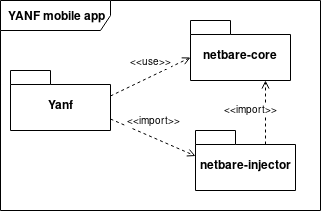
\includegraphics[width=0.5\textwidth]{Images/Diagrams/package-diagram.png}
    \caption{Package diagram - YANF}
    \label{fig:modview-package}
\end{figure}

\Autoref{fig:modview-blacklist} shows the class diagram for blacklisting certain domains. The classes are an abstraction of the disconnect.me list (described in \autoref{sec:disconnect-me}). The class \textit{MainActivity} is an implementation of an Android Activity which contains the UI logic. The class \textit{MozillaBlackList} contains all of the companies and the domains that are registered to them. The class \textit{BlackListLoader} is responsible for loading and deserializing JSON into Java objects.

\begin{figure}[H]
    \centering
    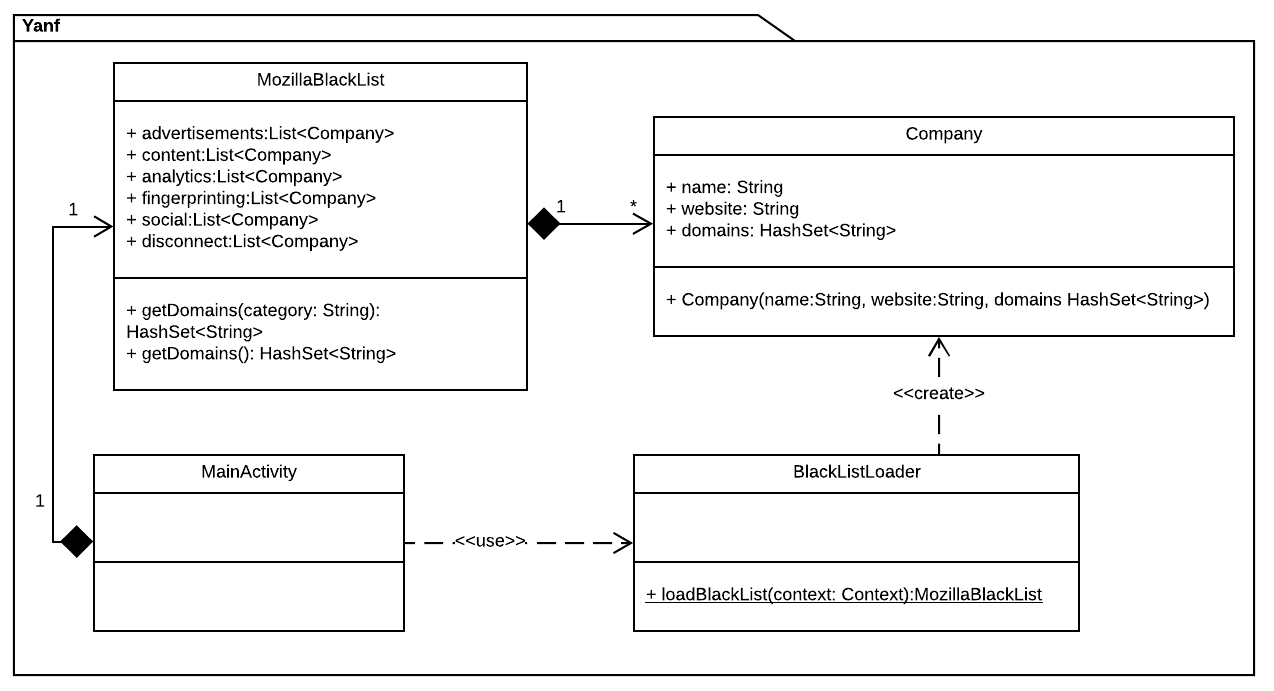
\includegraphics[width=1\textwidth]{Images/Diagrams/Class-diagram-BlackList-concept.png}
    \caption{Class diagram - Blacklist}
    \label{fig:modview-blacklist}
\end{figure}

\Autoref{fig:modview-injector} shows the class diagram for the custom HTTP injectors and how they are provided to NetBare. The two Injector-classes \textit{CookieInjector} and \textit{AdvertisementInjector} use some of the functionality provided by the abstract class \textit{SimpleHttpInjector}. All of methods from the interface are overridden by this abstract class but this is not shown in the diagram in order to reduce clutter. Two methods in both custom HTTP injectors are overridden; (1) sniffRequest() which returns a boolean whether or not any given request should be sniffed (i.e. injected) by the Injector and (2) onRequestInject() which handles the injection e.g. by removing the cookie-header or by blocking the request. The two injectors are provided to NetBare by (1) instantiating them in the class \textit{MainActivity} and (2) create an instance of \textit{HttpInterceptorFactory} through the static method createFactory() and (4) instantiate a default HTTP config through the class NetBareConfig and last (4) provide the NetBareConfig to the class NetBare throught the start() method which starts capturing of packets on the network with the use of Android's VPN service.

\begin{figure}[H]
    \centering
    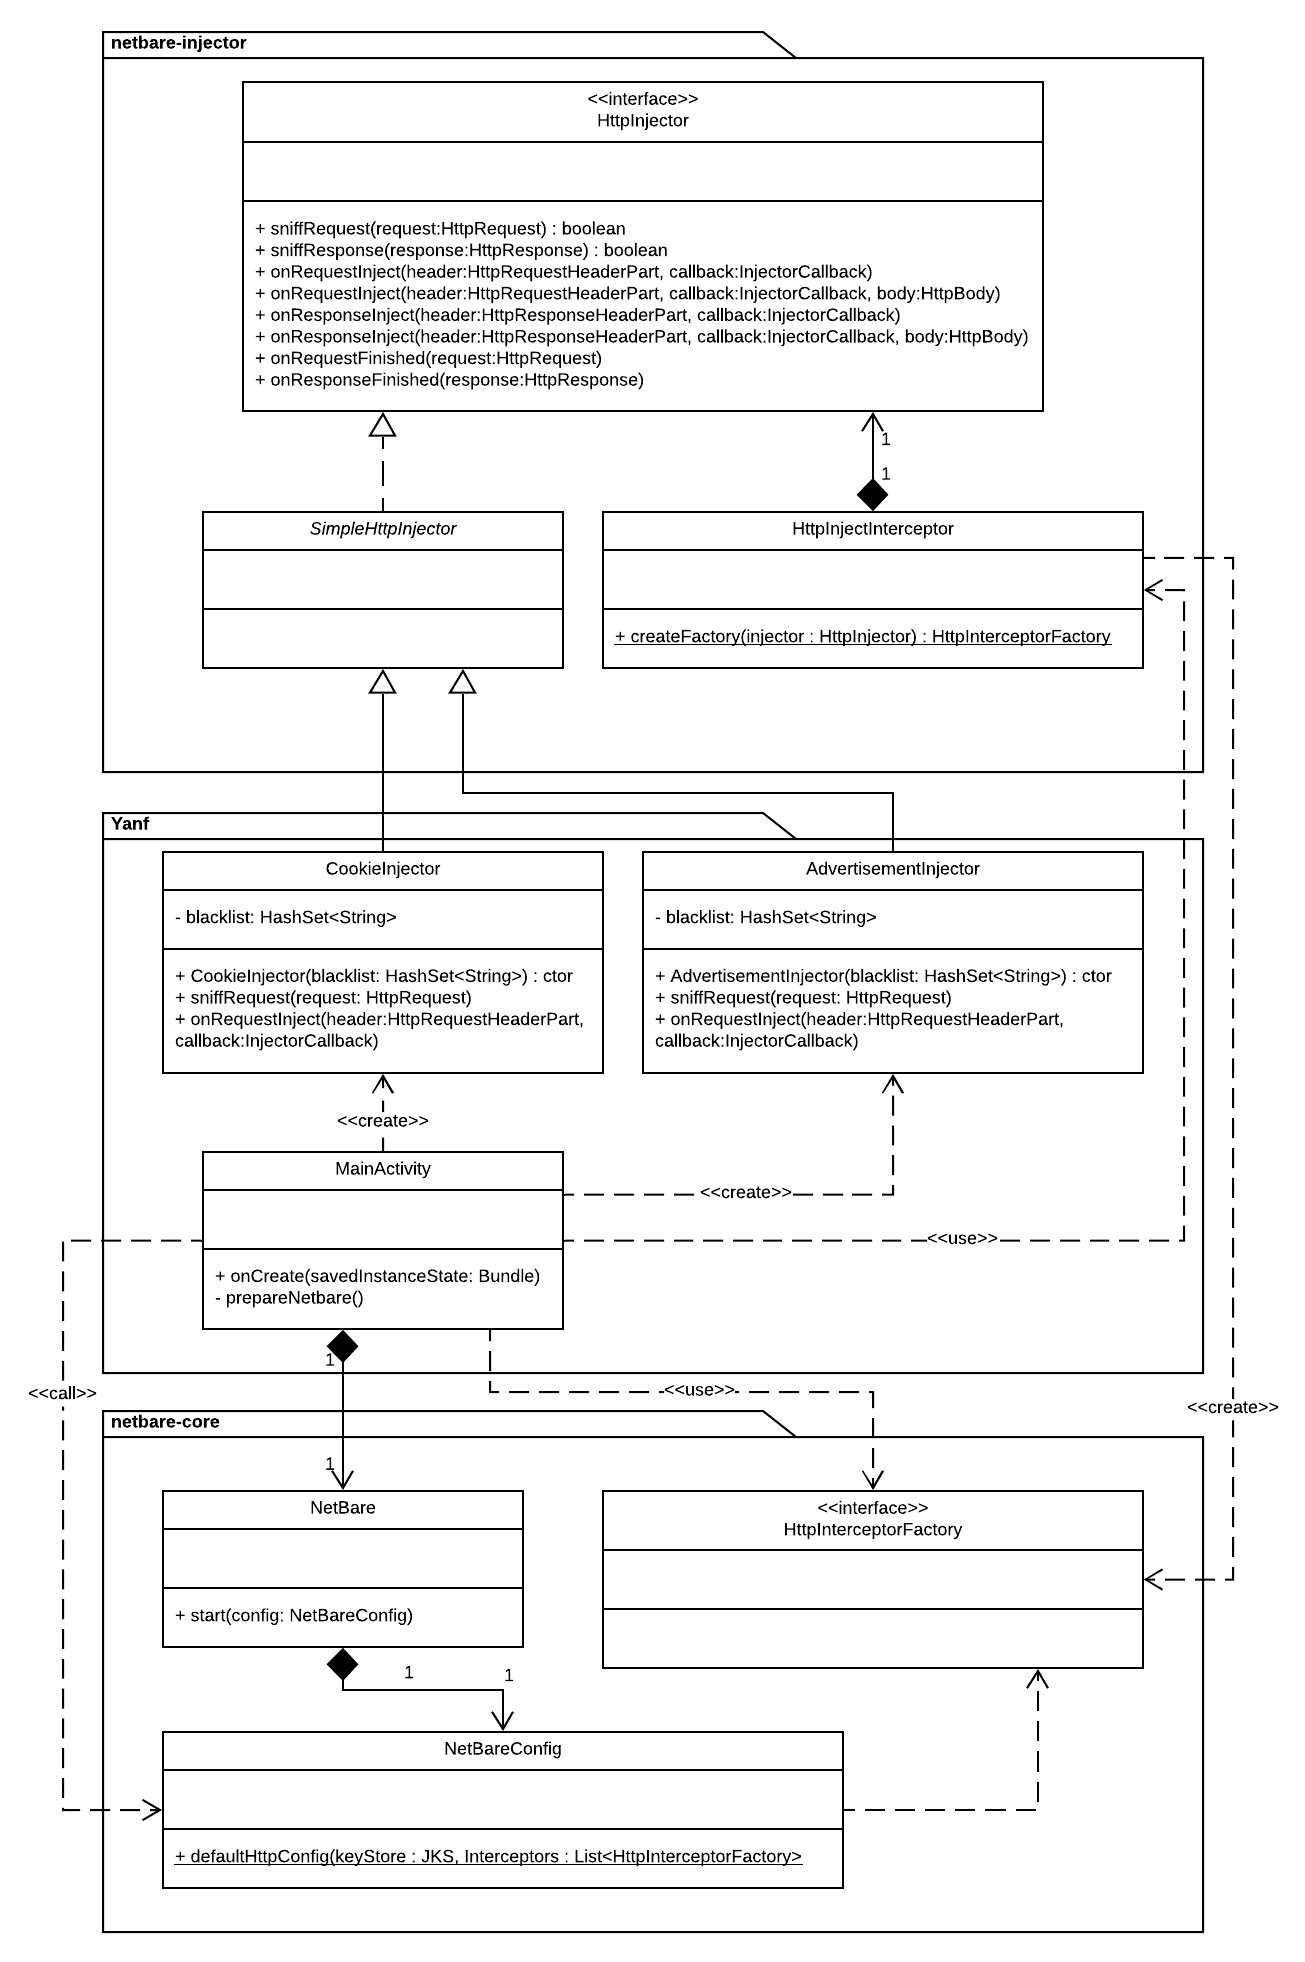
\includegraphics[width=1\textwidth]{Images/Diagrams/Class-diagram-injectors.png}
    \caption{Class diagram - Injectors}
    \label{fig:modview-injector}
\end{figure}


\subsection{Connector \& Component viewpoint}
Connector \& Component viewpoints are used to describe the functional behavior and communication of components in the system. Figure \ref{fig:ccdia} shows the components and how these are interconnected. YANF is the main component that relies on NetBare which encapsulates most functionality in a mobile app in a man-in-the-middle fashion. NetBare has three subcomponents that provides the communication between applications on the phone and with endpoints in order to inspect network packets. The \textit{User Interface} is an arbitrary application, that is requesting services of an arbitrary end point. The application sends regular TCP/IP requests but the traffic is sent through a local VPN which are able to redirect traffic through a local TCP proxy server. The proxy server then sends the traffic through a virtual gateway which contains a chain of interceptors. When the final interceptor has been processed, the request is finally sent to the end point.

\begin{figure}[H]
    \centering
    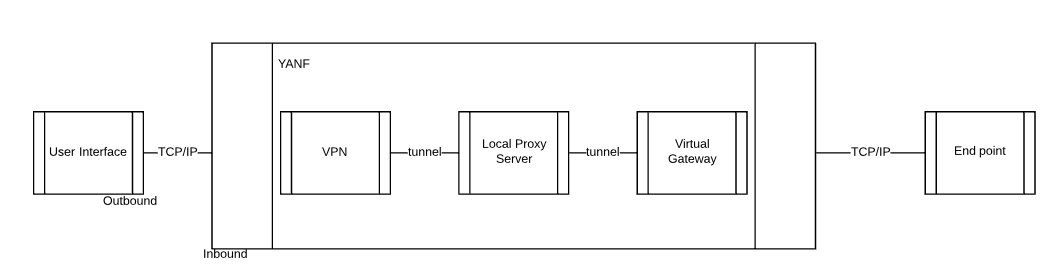
\includegraphics[width=\textwidth]{Images/Diagrams/ComponentDia.png}
    \caption{Component Viewpoint}
    \label{fig:ccdia}
\end{figure}

\Autoref{fig:request-sequence1} shows a sequence diagram for the flow of how an HTTP-request is sent from an arbitrary application on the phone to the gateway where it is eventually intercepted. All requests on the phone are transferred through \textit{NetBareThread} which is hosted inside an implementation of Android's \textit{VPNService} class. The request's header is then read in order to determine which proxy server that should handle the request based on the request's protocol type. In this case, the protocol type is TCP. The packet is thereafter forwarded to an \textit{TCPProxyServerForwarder} which modifies the original destination IP:port pair. The modified packet is once again written to the VPN output stream for outbound traffic. The roundtrip to the VPN makes sure that the modified packet is routed to the \textit{TCPProxyServer} instead of the original destination. Eventually the packet ends at the class \textit{NetBareVirtualGateway} which wraps the actual gateway where the packets are intercepted.

\begin{figure}[H]
    \centering
    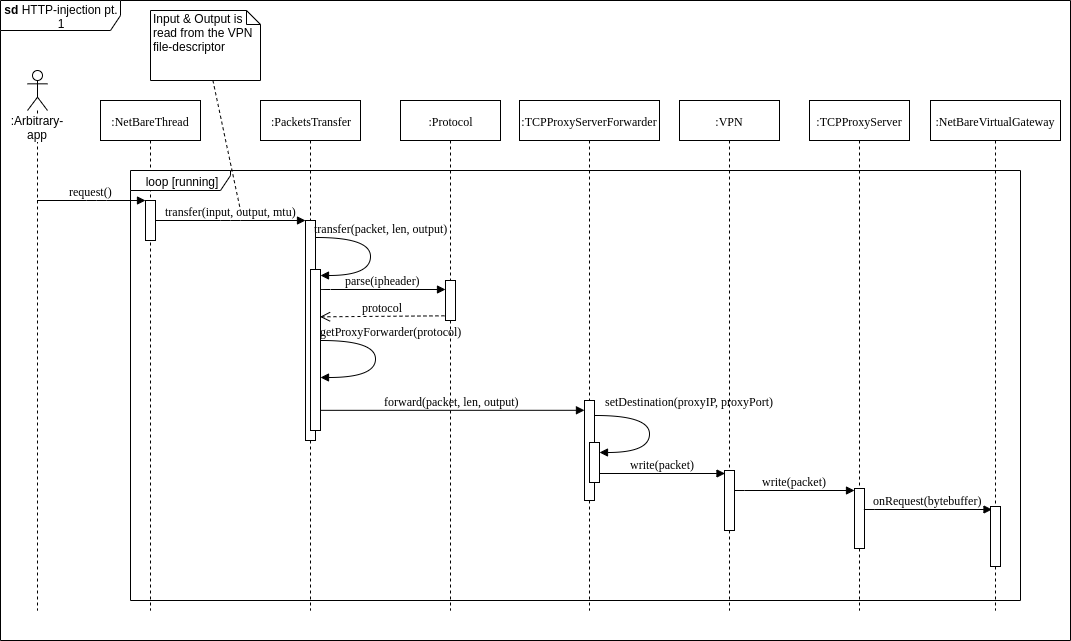
\includegraphics[width=\textwidth]{Images/Diagrams/request-sequence1.png}
    \caption{Sequence diagram - HTTP-injection pt. 1}
    \label{fig:request-sequence1}
\end{figure}

The interception chain is shown in the sequence diagram of \autoref{fig:request-sequence2}. The NetBare library makes use of the Chain-of-responsibility design pattern \cite{Gamma1994CreationalPatterns} which decouples the sender and receiver of a request - in this case the sender is the gateway and the receiver is the final endpoint. The sequence diagram starts with sending the request to the \textit{DefaultVirtualGateway} which then creates an instance of the \textit{InterceptorChain}. The chain-of-responsibility starts when the method \textit{process()} is called on the \textit{InterceptorChain}. All the interceptors in the chain is executed one after another and the HTTP packet is injected if the method \textit{sniffRequest()} returns \textit{true}. In the case of \textit{CookieInterceptor} the content of the HTTP header "Cookie" is removed. In the case of \textit{AdvertisementInterceptor}, the HTTP request is never sent to the terminal \textit{TunnelFlow} i.e. it is blocked. When there is no more interceptors left in the chain, the packet leaves the mobile devices through the class \textit{TunnelFlow} which is responsible for sending the injected packet to the remote host.

\begin{figure}[H]
    \centering
    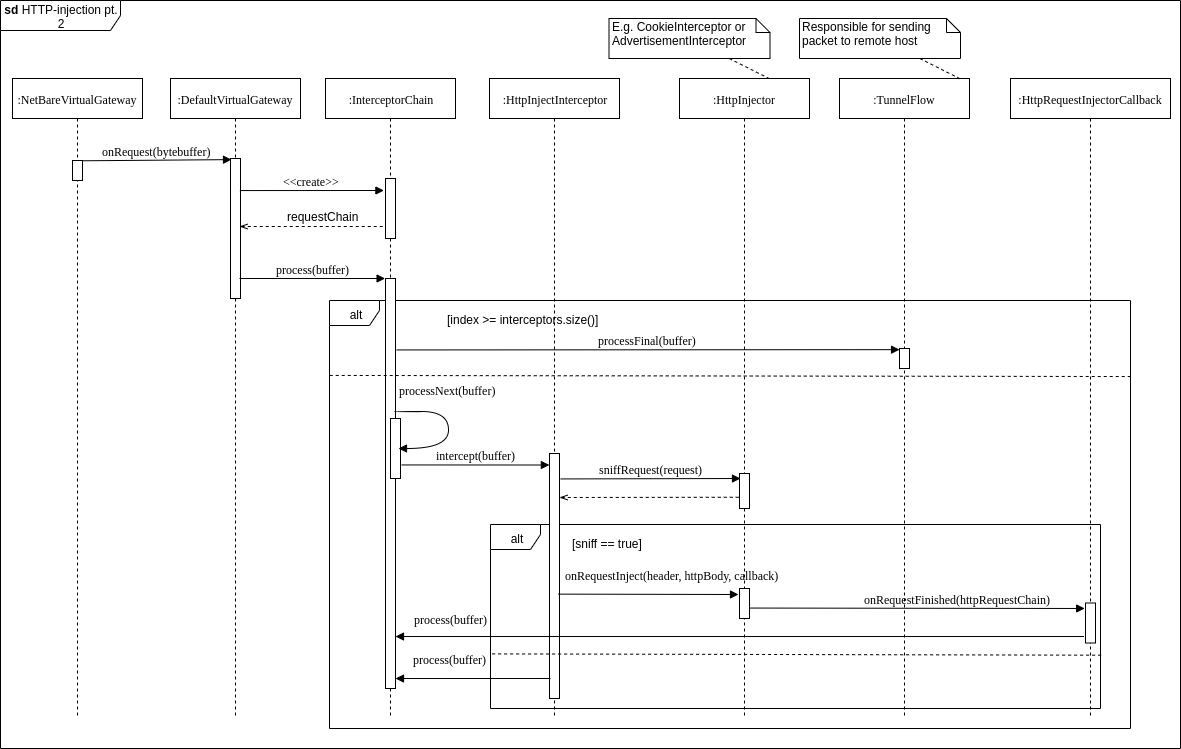
\includegraphics[width=\textwidth]{Images/Diagrams/request-sequence2.png}
    \caption{Sequence diagram - HTTP-injection pt. 2}
    \label{fig:request-sequence2}
\end{figure}


\subsection{Allocation Viewpoint} 
Allocation viewpoints are used to describe where software components are manifested and deployed onto physical hardware. YANF is compiled into an executable apk-file where all of the NetBare libraries are embedded within this single file.  \Autoref{fig:deployment} shows a deployment diagram of the YANF application where the device must be compatible with running Android apps targeted at API level 24 or higher.

\begin{figure}[H]
    \centering
    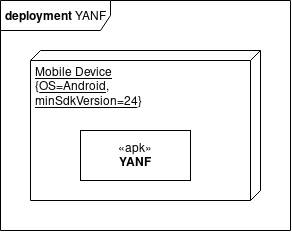
\includegraphics[width=0.45\textwidth]{Images/Diagrams/deployment.png}
    \caption{Deployment diagram - YANF}
    \label{fig:deployment}
\end{figure}



\end{document}